\section{OBSERVAÇÕES}
\label{sec:observacoes}

\subsection{Tratamento aos Dados}

Nesta sub-seção são apresentados resumidamente os tratamentos e pré-processamentos realizados sobre os dados da distribuição espaço-temporal dos casos de Influenza no ano de 2009 na cidade de Cascavel/PR, à obtenção de arquivos de entrada utilizados em simulações computacionais. Especificamente, os casos de Influenza são utilizados à obtenção dos arquivos de sazonalidade e distribuição de agentes infectados durante a simulação. As informações obtidas do arquivo de sazonalidade são utilizadas durante a operação de contato entre agentes suscetíveis e infectantes ao controle da taxa de infecção, de acordo com os casos reais observados. O arquivo de distribuição é utilizado à inserção de agentes infectados no ambiente durante a execução de simulações, sendo esses agentes responsáveis pelo início do processo infeccioso da doença. As posições nas quais estes agentes são inseridos correspondem às posições de casos reais de Influenza que foram georreferenciados. 

Aos dados dos $5.089$ casos de Influenza foram realizadas diversas atividades de pré-processamento. Inicialmente foram removidos aproximadamente $155$ casos não georreferenciados ou localizados em regiões não-urbanas da cidade de Cascavel/PR, como zonas rurais e distritos. Em sequência foram mantidos somente os casos com datas de ocorrência entre 17 de Junho e 31 de Dezembro de 2009, pois considerou-se estes casos mais significativos aos propósitos de simulação. Após estas operações restaram $4.658$ casos. Estes casos foram então agrupados por dia de ocorrência dos primeiros sintomas e são empregados à distribuição de agentes infectados durante a execução de simulações e ao cálculos das frações de sazonalidade. A Figura \ref{fig:casos} ilustra a distribuição espacial dos casos de Influenza durante o ano de 2009 e a Figura \ref{fig:casos_acumulados} ilustra o gráfico acumulado dos casos.

\begin{figure}[H]
  \centering
  \includegraphics[width=1\textwidth]{Figuras/Observacoes/Casos.png}
  \caption{Distribuição temporal dos casos de Influenza}
  \label{fig:casos}
\end{figure} 

\begin{figure}[H]
  \centering
  \includegraphics[width=1\textwidth]{Figuras/Observacoes/CasosAcumulados.png}
  \caption{Quantidade acumulada dos casos de Influenza}
  \label{fig:casos_acumulados}
\end{figure} 

O percentual de infecção dos agentes suscetíveis em contato com infectados é calculado utilizando-se três distintos parâmetros: os percentuais de infecção adotados às faixas etárias, a fração de sazonalidade do ciclo em que ocorre o contato e uma constante de sazonalidade. Todos esses percentuais são definidos em arquivos de configuração da simulação que são gerados ou manualmente ou por meio do \textit{software} SIMULA. Os percentuais de infecção por faixa etária e a constante de sazonalidade foram definidos de forma empírica por meio de execução de testes. As frações de sazonalidade por ciclo foram definidos com base na distribuição temporal acumulada dos casos de Influenza durante o ano de 2009. 

Assim como realizado por outros autores como (Dalgiç et al, 2017) e (Arduin et al, 2017) foi empregado um fator de escala, a constante de sazonalidade, com média de $0.83$ para calibrar o modelo, visto que alguns parâmetros utilizados tem origem em modelos compartimentais e não em modelos multiagentes, de modo que eles não são totalmente satisfatórios para serem utilizados diretamente no modelo apresentado.

A Figura \ref{fig:curva_teorica} ilustra o ajuste realizado aos casos de Influenza utilizando a função \textit{curve\_fit} do pacote \textit{optimize} da biblioteca \textit{Python} \textit{Scipy} e empregando uma função tipo logística acumulada, em que os pontos em verde representam a quantidade normalizada de casos acumulados e em vermelho é ilustrada a curva da equação ajustada. A função utiliza o método dos quadrados mínimos não linear.

\begin{figure}[H]
  \centering
  \includegraphics[width=0.9\textwidth]{Figuras/Observacoes/Teorico.png}
  \caption{Ajuste aos casos de Influenza utilizando uma função logística acumulada}
  \label{fig:curva_teorica}
\end{figure} 

O efeito de saturação que ocorre na doença modelada, decorrente de efeitos ambientais, de transmissão e contato, entre outros, foi mimetizado por meio do complemento da função logística acumulada. Utilizou-se a função $F(t)=1-L(t)$, em que $L(t)$ é a função logística que foi previamente ajustada aos dados, apresentada na Figura \ref{fig:curva_teorica}, para ponderar a força de infecção ao longo do tempo $t$ da simulação. Na Figura \ref{fig:percentuais_sazonalidade} é apresentada a curva resultante dos cálculos dos complementos, que são utilizados como frações de sazonalidade durante a simulação à obtenção dos percentuais de infecção de agentes suscetíveis em contato com infectados. 

\begin{figure}[H]
  \centering
  \includegraphics[width=1\textwidth]{Figuras/Observacoes/Sazonalidade.png}
  \caption{Distribuição temporal das frações de sazonalidade}
  \label{fig:percentuais_sazonalidade}
\end{figure} 

O arquivo de distribuição de agentes infectados ao longo da simulação é gerado pela função \textit{salvarArquivoDistribuicaoHumanos}, que é ilustrada no Código \ref{cod:salvarArquivoDistribuicaoHumanos}, Algoritmo \ref{alg:salvarArquivoDistribuicaoHumanos} e Figura \ref{fig:salvarArquivoDistribuicaoHumanos}. A função emprega percentuais de casos utilizados e frações de machos e fêmeas para cada faixa etária, de acordo com informações provenientes do banco de dados. Foram utilizadas como base as faixas etárias definidas pelo IBGE, que classificam os indivíduos de acordo com sua idade, como apresentado na Tabela \ref{tab:faixasEtariasIBGE}.  

\begin{table}[H]
\centering
\begin{tabular}{c|c}
 \textbf{Idade} 	& \textbf{Faixa Etária}	\\ \hline
 Menor que 15 anos 	& Criança		\\
 Entre 15 e 24 anos 	& Jovem			\\
 Entre 25 e 59 anos 	& Adulto		\\
 Maior que 59 anos 	& Idosos		\\
\end{tabular}
\caption{Tabela das faixas etárias definidas pelo IBGE.}
\label{tab:faixasEtariasIBGE}
\end{table}

Um aspecto importante é o fato de que a dinâmica do espalhamento não dependa de apenas um conjunto de indivíduos infectados distribuídos inicialmente, como em modelos compartimentais. Considerou-se que a distribuição de infectados não é espaço-temporalmente local, mas sim realizada ao longo da simulação em posições escolhidas aleatoriamente. Essa estratégia baseou-se na suposição de que os casos da doença surgem de forma não concentrada ao longo do espaço, assim como contemplar os casos assintomáticos ou as subnotificações da doença que, no entanto, são fontes relevantes de infectados à propagação da doença. Na modelagem realizada escolheu-se inserir 3\% dos casos ao longo da simulação à quantidade de infectantes observados por dia, realizando um mapeamento entre os dias de ocorrência dos casos e os ciclos de simulação.

Para as crianças, $51\%$ são masculinos e $49\%$ são femininos. Para os jovens, $50\%$ são masculinos e $50\%$ são femininos. Para os adultos, $48\%$ são masculinos e $52\%$ são femininos. Por fim, para os idosos, $45\%$ são masculinos e $55\%$ são femininos. Na escolha dos casos que serão utilizados inicialmente o conjunto de todos os casos é agrupado por dia de ocorrência. Em seguida, para cada dia são mantidos $3\%$ dos casos. Os casos são então agrupados por faixa etária e os percentuais apresentados anteriormente são utilizados à atribuição aleatória dos sexos. O passo final do algoritmo consiste em atribuir uma posição para a inserção do agente no ambiente, já que os pontos originais dos casos georreferenciados podem não estar presentes no conjunto de pontos interpolados no ambiente. Neste caso, o ponto do ambiente que é mais próximo aquele do caso original é escolhido, considerando-se a distância euclidiana entre eles. 

A Figura \ref{fig:funcoes_logistica} ilustra as curvas obtidas por meio de ajustes realizados aos dados. As quantidades de casos de infecção reais por dia foram normalizados no intervalo $[0.0, 1.0]$ e são ilustrados na cor verde. À esses dados foi ajustada uma equação tipo Logística Acumulada, que é ilustrada na cor vermelha. Na cor marrom é ilustrada a equação ajustada aos resultados obtidos por meio de simulação computacional e os pontos em azul apresentam as quantidades de casos de infecção simulados normalizados no intervalo $[0.0, 1.0]$. 

\begin{figure}[H]
  \centering
  \includegraphics[width=1\textwidth]{Figuras/Observacoes/Logistica.png}
  \caption{Curvas das equações tipo Logística Acumulada ajustadas aos dados reais e simulados. }
  \label{fig:funcoes_logistica}
\end{figure} 

\subsection{Distribuição Inicial por Quadras ou Pontos}

Nas rotinas de distribuição inicial ou inserção durante a execução, duas abordagens podem ser implementadas à escolha das posições iniciais dos agentes: por quadras ou por pontos. Na abordagem por quadras, escolhe-se primeiramente, de forma aleatória, uma quadra do ambiente. Em seguida são escolhidos aleatoriamente um lote pertencente à esta quadra e por fim uma posição pertencente à este lote. Na abordagem por pontos escolhe-se diretamente uma posição qualquer pertencente ao ambiente. 

Considerando as quantidades ilustradas na Tabela \ref{tab:quant_quadras_pontos}, a Tabela \ref{tab:perc_quadras_pontos} apresenta as probabilidades de escolha de um particular tipo de ponto ou quadra. É possível concluir que, para o ambiente de Boa Vista da Aparecida, empregando a abordagem por quadras, a probabilidade de um agente ocupar uma posição urbana é maior. Já com a abordagem por pontos, a probabilidade é maior para pontos rurais. Para o ambiente de Cascavel, com a abordagem por quadras, a probabilidade da escolha de pontos de quadras urbanas é maior. Já para a abordagem por pontos, a probabilidade de escolha de pontos de rua é maior. 

\begin{table}[H]
\centering
\begin{tabular}{c|c|c}
				& \textbf{Cascavel}		& \textbf{Boa Vista da Aparecida} 	\\ \hline
 \textbf{Quadras Urbanas}	& $31$				& $152$	  				\\
 \textbf{Quadras Rurais} 	& $0$				& $10$	  				\\
 \textbf{Quadras de Rua}	& $1$				& $1$	  				\\ \hline
 \textbf{Pontos Urbanos}	& $66.300$			& $39.767$	  			\\ 
 \textbf{Pontos Rurais}		& $0$				& $85.217$  				\\
 \textbf{Pontos de Rua}		& $103.269$			& $12.759$  				\\
 \end{tabular}
\caption{Tabela indicando as quantidades de cada tipo de quadra e pontos nos ambientes de Cascavel e Boa Vista da Aparecida. }
\label{tab:quant_quadras_pontos}
\end{table}

\begin{table}[H]
\centering
\begin{tabular}{c|c|c}
				& \textbf{Cascavel}		& \textbf{Boa Vista da Aparecida} 	\\ \hline
 \textbf{Quadras Urbanas}	& $0,9688$			& $0,9325$	  			\\
 \textbf{Quadras Rurais} 	& $0$				& $0,0614$	  			\\
 \textbf{Quadras de Rua}	& $0,0312$			& $0,0061$	  			\\ \hline
 \textbf{Pontos Urbanos}	& $0,391$			& $0,2887$	  			\\ 
 \textbf{Pontos Rurais}		& $0$				& $0,6187$  				\\
 \textbf{Pontos de Rua}		& $0,609$			& $0,0926$  				\\
 \end{tabular}
\caption{Tabela indicando as probabilidades de escolha de cada tipo de quadra e pontos nos ambientes de Cascavel e Boa Vista da Aparecida. }
\label{tab:perc_quadras_pontos}
\end{table}

A escolha de uma particular abordagem influencia fortemente a rotina de distribuição de agentes pois pode levar à concentração de agentes em determinadas regiões, como urbanas, de ruas ou rurais. Esta concentração pode aumentar ou diminuir a quantidade de contatos realizados entre agentes e consequentemente afeta a dinâmica de transmissão da doença espaço-temporalmente. 

Considerando que os agentes distribuídos utilizando a abordagem por quadras têm probabilidade maior de concentrar-se em posições pertencentes à áreas urbanas do ambiente, optou-se por utilizar esta abordagem como padrão nas implementações realizadas, pois considera-se que a concentração de agentes em posições urbanas é mais relevante e interessante aos propósitos atuais de modelagem. 

\subsection{Discussões sobre Monte Carlo Espacial}

Com o objetivo de mimetizar as saídas tipo Monte Carlo obtidas a partir das quantidades de agentes ao longo do tempo de simulação desenvolveu-se um programa ao processamento de arquivos de saídas espaciais, provenientes da execução de simulações individuais, à confecção de saídas espaciais acumuladas tipo Monte Carlo. A estratégia de Monte Carlo à solução espaço-temporal foi realizada considerando-se os novos casos de infectantes, por ciclo e por simulação individual. Denomina-se simulação individual aquelas simulações que são utilizadas à composição de uma simulação Monte Carlo. 

Após a execução de todas as simulações individuais toma-se a divisão inteira da quantidade total de posições com agentes no estado infectante, pela quantidade de simulações, que são ordenadas em ordem decrescente. Em sequência toma-se os acumulados, por ciclo, para todas as simulações. Do vetor resultante dessa operação, toma-se os $n$ primeiros elementos da quantidade obtida na divisão inteira realizada anteriormente. Após a cada ciclo realiza-se uma operação entre os vetores das médias dos elementos que são gerados à cada ciclo, que por meio de uma soma parcial à cada passo de tempo, gera um vetor de casos acumulados por posição. Do vetor de soma parcial é realizada divisão de inteiros buscando avaliar a quantidade de elementos que deve constar no vetor de saída não acumulada. Neste vetor é utilizado o mesmo critério anteriormente discutido à escolha das posições, que são utilizadas à obtenção do arquivo de saída final, na forma de casos acumulados no espaço e no tempo. O Código \ref{cod:espacial_media} e Algoritmo \ref{alg:espacial_media} apresentam o código-fonte e pseudo-código do programa responsável pela geração das saídas espaciais acumuladas tipo Monte Carlo. 

\lstinputlisting[title=espacial\_media4.cpp, captionpos=b, label=cod:espacial_media, language=C++]{Codigos/Observacoes/espacial_media4.cpp}

\begin{algorithm}[H]
  \SetAlgoLined   
  \input{Codigos/Observacoes/espacial_media4.txt}
  \caption{\textsc{Algoritmo Monte Carlo Espacial}}
  \label{alg:espacial_media}
\end{algorithm}

Para demonstrar o algoritmo de geração de saídas espaciais tipo Monte Carlo é apresentado abaixo um exemplo de sua aplicação em um conjunto de saídas fictício. A Figura \ref{fig:monte_carlo_espacial_1} ilustra as saídas utilizadas, em que considerou-se um ambiente hipotético com 16 posições, uma simulação Monte Carlo composta por 3 simulações individuais, cada uma com duração de 6 ciclos. Nas linhas intituladas \textit{"Simulação"} são apresentados horizontalmente os resultados espaciais das simulações para os 6 ciclos de tempo considerados. Os ciclos de tempo intitulam as colunas como \textit{"Tempo"} e apresentam verticalmente os resultados para determinados ciclos nas 3 simulações. As posições marcadas com \textit{"X"} representam posições com a presença de pelo menos um agente infectado, assim como posições sem marcação indicam que determinada posição não apresentou agente infectado naquele ciclo de tempo. Cada posição da matriz apresenta um identificador numérico que pode ser observado em seu canto superior esquerdo, que será utilizado para referenciar cada posição. 

\begin{figure}[H]
  \centering
  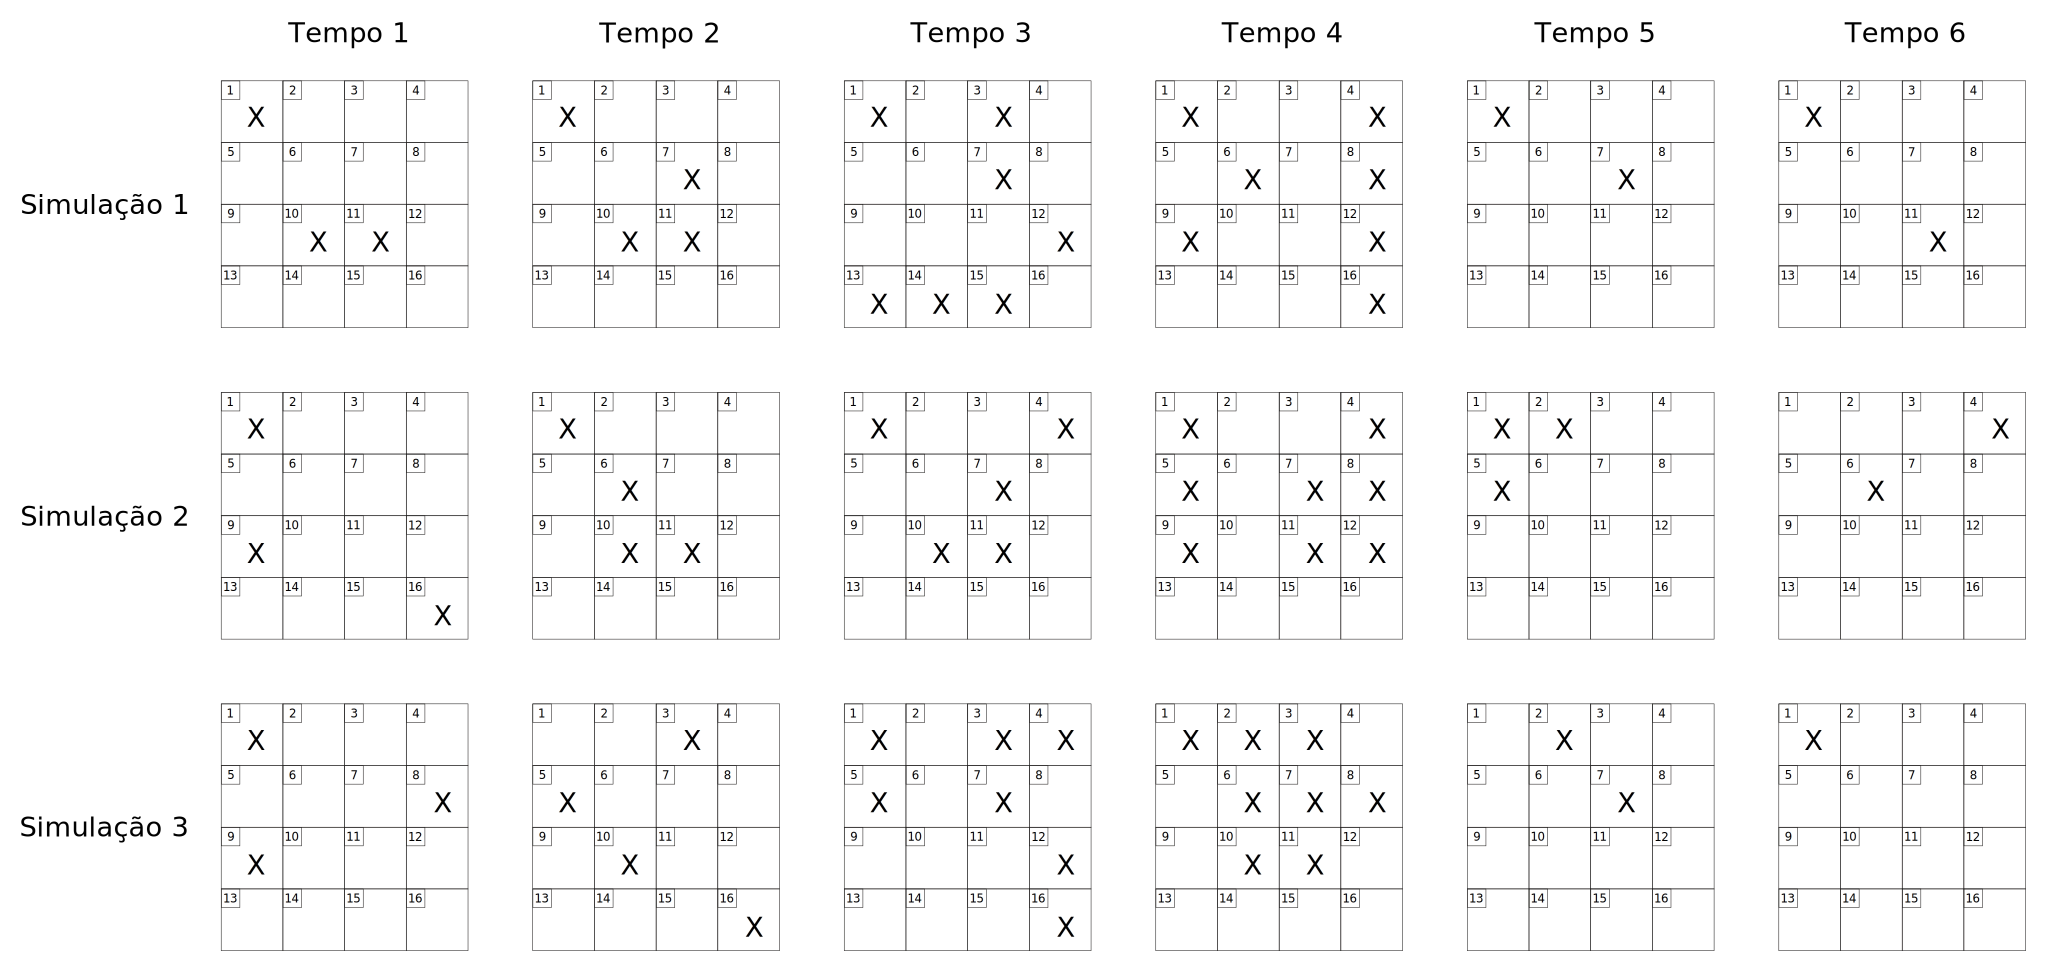
\includegraphics[width=1\textwidth]{Figuras/Observacoes/MonteCarloEspacial/folha1.png}
  \caption{Saídas espaciais fictícias. }
  \label{fig:monte_carlo_espacial_1}
\end{figure} 

Na Figura \ref{fig:monte_carlo_espacial_2} são apresentados dois conjuntos de resultados espaciais. O conjunto nomeado \textit{"Soma das Simulações"} apresenta as somas por ciclo das matrizes apresentadas na Figura \ref{fig:monte_carlo_espacial_1}. A soma entre as matrizes é realizada elemento a elemento. Para exemplificar, no \textit{"Tempo 1"}, a posição 1 da matriz de saída possui o valor 3 pois resultou da soma entre as posições 1, do \textit{"Tempo 1"}, das 3 simulações individuais. Da mesma forma, a posição 2 do mesmo tempo possui o valor 2 resultante da soma das posições 9 das simulações 2 e 3. 

O conjunto nomeado \textit{"Média das Simulações"} apresenta uma média espacial obtida do conjunto \textit{"Soma das Simulações"}. Inicialmente, é realizada uma soma dos valores presentes na tabela, resultando em um único número por matriz. Este número é então dividido pela quantidade de simulações. Desprezando-se o resto da divisão, o resultado determina a quantidade de posições que serão mantidas. Escolhe-se as posições que tenham maior valor na matriz de soma. A escolha é aleatória nos casos em que as posições apresentam valor 1. Para exemplificar, no \textit{"Tempo 1"}, a soma dos valores apresentados na matriz é 9. Divide-se este valor por 3, que é a quantidade de simulações, resultado em 3, que é a quantidade de posições que serão mantidas. Escolhe-se então as posições 1 e 9, pois têm os maiores valores da matriz. Por último escolhe-se também a posição 10, mas poderiam ser escolhidas em seu lugar as posições 8, 11 e 16. Da mesma forma, no \textit{"Tempo 2"}, a soma dos valores apresentados na matriz é 12. Divide-se este valor por 3 resultando em 4. Escolhe-se então as posições 1, 10 e 11, pois têm os maiores valores da matriz. Por último escolhe-se também a posição 3, mas poderiam ser escolhidas em seu lugar as posições 5, 6, 7 e 16.

\begin{figure}[H]
  \centering
  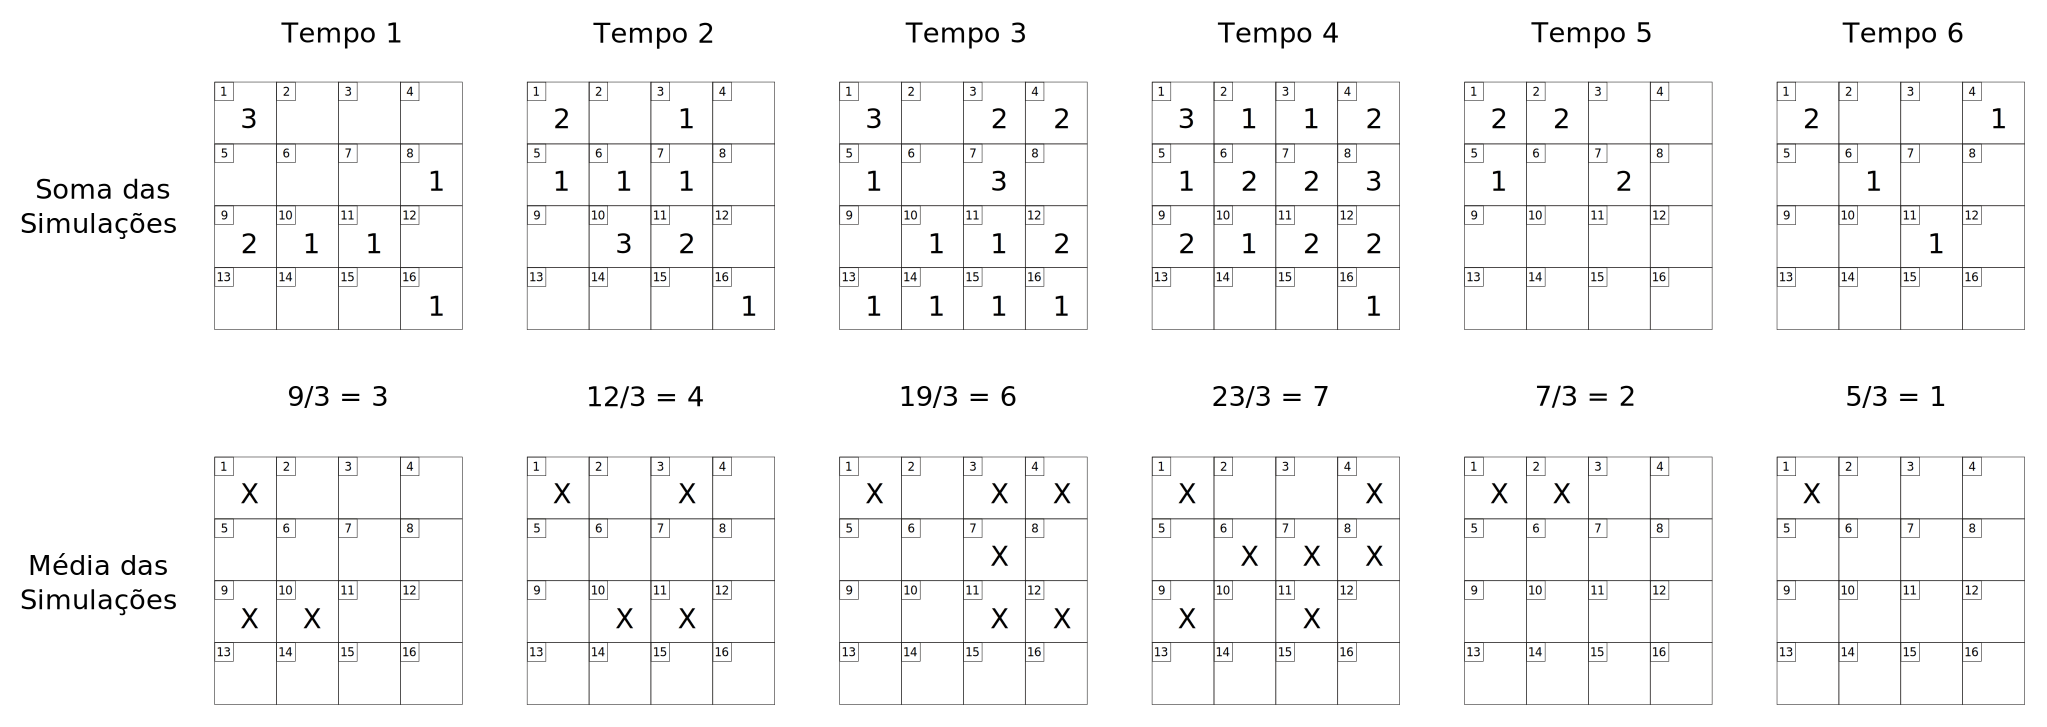
\includegraphics[width=1\textwidth]{Figuras/Observacoes/MonteCarloEspacial/folha2.png}
  \caption{Matrizes de soma e média das simulações. }
  \label{fig:monte_carlo_espacial_2}
\end{figure} 

Na Figura \ref{fig:monte_carlo_espacial_3} são apresentados três conjuntos de resultados espaciais. O conjunto nomeado \textit{"Acumulado das Médias das Simulações"} apresenta a soma parcial, ciclo a ciclo, do conjunto \textit{"Média das Simulações"} apresentado na Figura \ref{fig:monte_carlo_espacial_2}. Para exemplificar a operação de soma parcial, a matriz resultante apresentada no \textit{"Tempo 4"} do conjunto \textit{"Acumulado das Médias das Simulações"} é resultado da soma entre as matrizes \textit{"Tempo 1"}, \textit{"Tempo 2"}, \textit{"Tempo 3"} e \textit{"Tempo 4"} do conjunto \textit{"Média das Simulações"}. O mesmo processo é realizado para os outros ciclos de tempo. 

O conjunto \textit{"Média do Acumulado"} é resultado da média espacial do conjunto \textit{"Acumulado das Médias das Simulações"}, empregando ideia similar aquela utilizada à obtenção do conjunto \textit{"Médias das Simulações"} apresentado na Figura \ref{fig:monte_carlo_espacial_2}. Desta ideia aplicada anteriormente, o divisor da soma total dos elementos da matriz é alterado, utilizando no lugar da quantidade de simulações o identificador numérico do ciclo ou tempo, iniciando em 1. Para exemplificar, a matriz resultante apresentada no \textit{"Tempo 6"} do conjunto \textit{"Média do Acumulado"} é resultante da escolha dos elementos 1, 7 e 11 da matriz no \textit{"Tempo 6"} do conjunto \textit{"Acumulado das Médias das Simulações"}. Escolheu-se 3 elementos pois é o resultado da soma dos elementos da matriz, que é 23, dividido pelo identificador numérico do ciclo, que é 6. No lugar do elemento 7 poderiam ser escolhidos os elementos 3, 4, 9 e 10 pois têm mesmo valor. 

O conjunto \textit{"Acumulado Final"} resulta do processamento do conjunto \textit{"Média do Acumulado"}, aplicando ideia similar aquela empregada à obtenção do conjunto \textit{"Acumulado das Médias das Simulações"}, realizando-se a soma parcial, ciclo a ciclo, do conjunto de entrada. 

\begin{figure}[H]
  \centering
  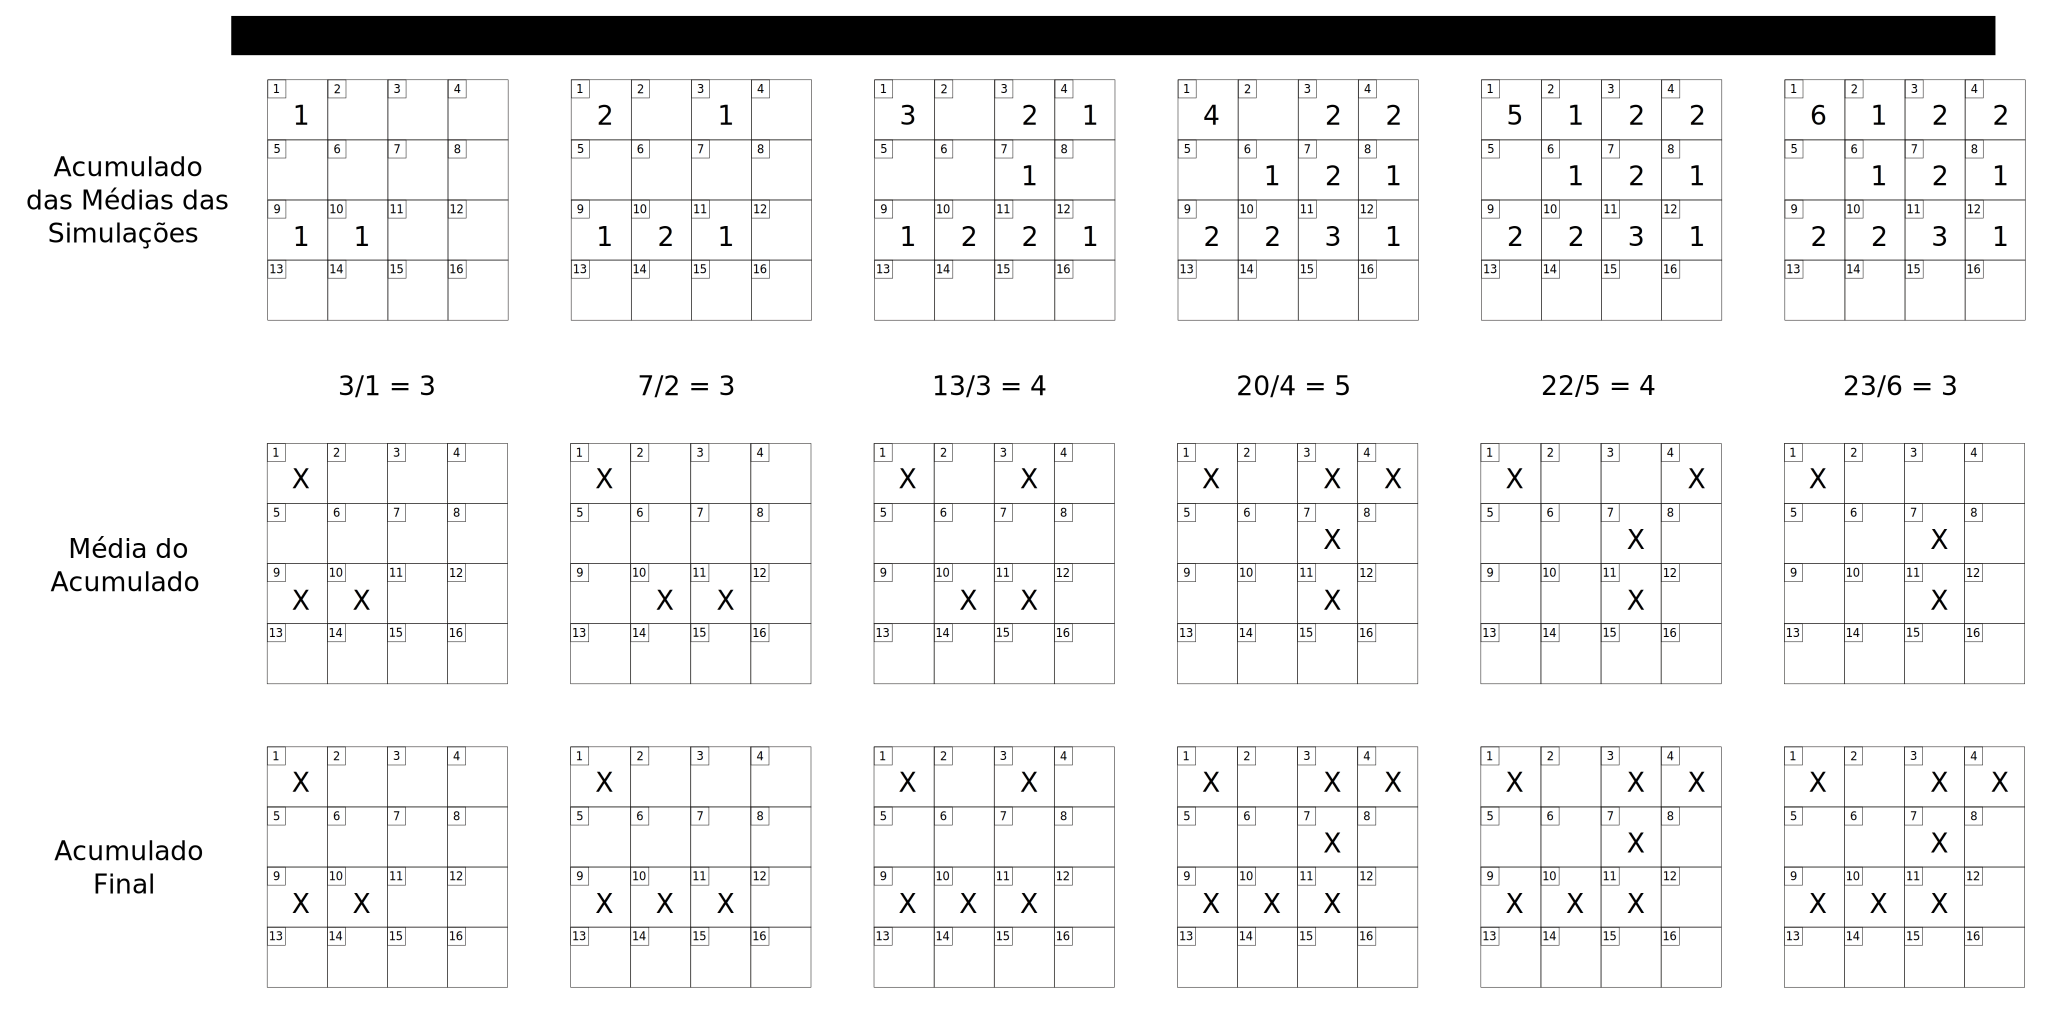
\includegraphics[width=1\textwidth]{Figuras/Observacoes/MonteCarloEspacial/folha3.png}
  \caption{Matrizes de acumulado das médias das simulações, da média do acumulado e do acumulado final. }
  \label{fig:monte_carlo_espacial_3}
\end{figure} 

\subsection{Discussões sobre Implementações Paralelas em CPU e GPU} 

À implementação do sistema de simulação utiliza-se a linguagem de programação C++ e a biblioteca \textit{CUDA} \textit{Thrust}, que é baseada na biblioteca padrão da linguagem e disponibiliza estruturas de dados e algoritmos de alto nível à implementação de aplicações paralelas. Desta forma, a biblioteca é de grande auxílio à programação de sistemas paralelos, pois aumenta a produtividade do programador dispensando-o de preocupar-se com detalhes de baixo nível como alocações, cópias de memória e definição da quantidade de \textit{threads} utilizadas na execução. 

Durante o processo de implementação optou-se por manter os diversos algoritmos necessários à simulação organizados em operadores distintos. Esta organização facilitou o processo de desenvolvimento utilizando a biblioteca \textit{Thrust}, que oferece interfaces adequadas à abordagem em operadores por meio de predicados, e contribuiu à estruturação geral do código-fonte, mantendo algoritmos relacionados encapsulados em operadores próprios. 

Em sequência são apresentados os principais \textit{headers} disponibilizados pela biblioteca que são utilizados na implementação do sistema. 

\begin{itemize}
 \item \textbf{device\_vector.h:} Neste arquivo é definida a classe \textit{device\_vector}, que é a principal estrutura de dados utilizada na simulação. É responsável pelo armazenamento de conjuntos de elementos e é baseada na estrutura \textit{std::vector} definida na biblioteca padrão da linguagem. 
 \item \textbf{random.h:} Neste arquivo são definidas classes empregadas na geração de números aleatórios. São utilizadas as classes \textit{default\_random\_engine} e \textit{uniform\_real\_distribution} à geração de números aleatórios reais empregando uma distribuição uniforme. 
 \item \textbf{count.h:} Neste arquivo são definidas as funções \textit{count} e \textit{count\_if}, que são utilizadas para obter a quantidade de elementos de um conjunto que atendem à um determinado predicado. 
 \item \textbf{iterator.h:} Neste arquivo são definidas estruturas auxiliares à iteração sobre conjuntos utilizando índices, como iteradores constantes, contadores e outros, que emulam os identificadores das \textit{threads}. São utilizados os iteradores \textit{counting\_iterator} e \textit{constant\_iterator}. 
 \item \textbf{reduce.h:} Neste arquivo é definida a função \textit{reduce\_by\_key}, que é empregada durante a atualização dos índices dos agentes. 
 \item \textbf{replace.h:} Neste arquivo é definida a função \textit{replace}, que é utilizada para substituir elementos em um conjunto por outros. 
 \item \textbf{scan.h:} Neste arquivo é definida a função \textit{inclusive\_scan}, que é utilizada na atualização dos índices dos agentes. 
 \item \textbf{set\_operations.h:} Neste arquivo é definida a função \textit{set\_difference}, que calcula o conjunto diferença entre dois outros conjuntos. 
 \item \textbf{sort.h:} Neste arquivo é definida a função \textit{sort}, que é utilizada para ordenação de conjuntos de elementos de acordo com um critério. 
 \item \textbf{transform.h e transform\_reduce.h:} Nestes arquivos são definidas as funções \textit{transform} e \textit{transform\_reduce}, que são utilizadas para modificar um conjunto de elementos por meio de outra função. 
 \item \textbf{copy.h:} Neste arquivo é definida a função \textit{copy}, que é empregada à cópia de dados entre conjuntos de elementos. Esta função também pode ser utilizada à transferência de dados entre CPU e GPU. 
 \item \textbf{for\_each.h:} Neste arquivo é definida a função \textit{for\_each\_n}, que é amplamente utilizada para a execução paralela dos operadores sobre a população de agentes ou sobre o ambiente. 
 \item \textbf{tuple.h:} Neste arquivo é definida a estrutura \textit{tuple}, que é utilizada como estrutura de dados auxiliar em alguns trechos do código-fonte. 
 \item \textbf{functional.h:} Neste arquivo são definidos diversos predicados que podem ser utilizados em conjunto com os algoritmos definidos pela biblioteca. Efetivamente, somente a função \textit{plus} é utilizada na atual implementação. 
 \item \textbf{partition.h:} Neste arquivo é definida a função \textit{partition}, que é utilizada para particionar um conjunto de elementos de acordo com um predicado. 
\end{itemize}

Além dos algoritmos e estruturas apresentados a função \textit{raw\_pointer\_cast} é utilizada à obtenção de \textit{raw pointers} de estruturas de alto nível como \textit{device\_vectors}. Esta função retorna um ponteiro direto aos dados de uma estrutura de alto nível e é especialmente útil à passagem de parâmetros aos métodos dos operadores implementados na simulação. É fundamental ao estilo de implementação adotado pois a classe \textit{device\_vector} não pode ser utilizada em trechos de códigos internos à \textit{kernels CUDA}, como é o caso dos operadores. Assim, um ponteiro direto aos dados é passado à função e é acessado de maneira similar aquela realizada para \textit{arrays} na linguagem C. 

A biblioteca viabiliza ainda a execução do código tanto em GPU quanto em CPU, por meio de diferentes \textit{backends} que podem ser selecionados com \textit{flags} específicas informadas ao compilador, dispensando a necessidade de implementação de versões distintas para execução em GPU e CPU. Um tutorial sobre a escolha do \textit{backend} na biblioteca \textit{Thrust} pode ser encontrado em \url{https://github.com/thrust/thrust/wiki/Device-Backends}. Atualmente são utilizados os \textit{backends} \textit{CUDA} e \textit{OpenMP} para execução em GPU e CPU, respectivamente, e são definidos dois \textit{Makefiles} distintos, que informam ao compilador as \textit{flags} correspondentes visando a execução em GPU ou CPU. 

\subsection{Outras Discussões Pertinentes}

Os parâmetros utilizados na execução de testes são baseados naqueles apresentados nos artigos... {\color{red} REFERENCIAR ARTIGOS. }

A aplicação de um atraso (\textit{delay}) no vetor de percentuais de sazonalidade somente desempenha o papel de mover a curva acumulada dos agentes infectantes pelo eixo $x$. 

A distribuição de infectantes durante a simulação tem justificativas no artigo (Miksch et. al, 2011). {\color{red} REFERENCIAR ARTIGO. }

\newpage